

\chapter{Noise Reduction through De-Whitening Filter}

\section{Principle of De-Whitening Filter}
De-Whitening Filter is an equalizer type analog filter. It has a specific frequency response such that 


\section{Circuit Design}

%\begin{figure}[hbt!]
%\centering
\begin{sidewaysfigure}
%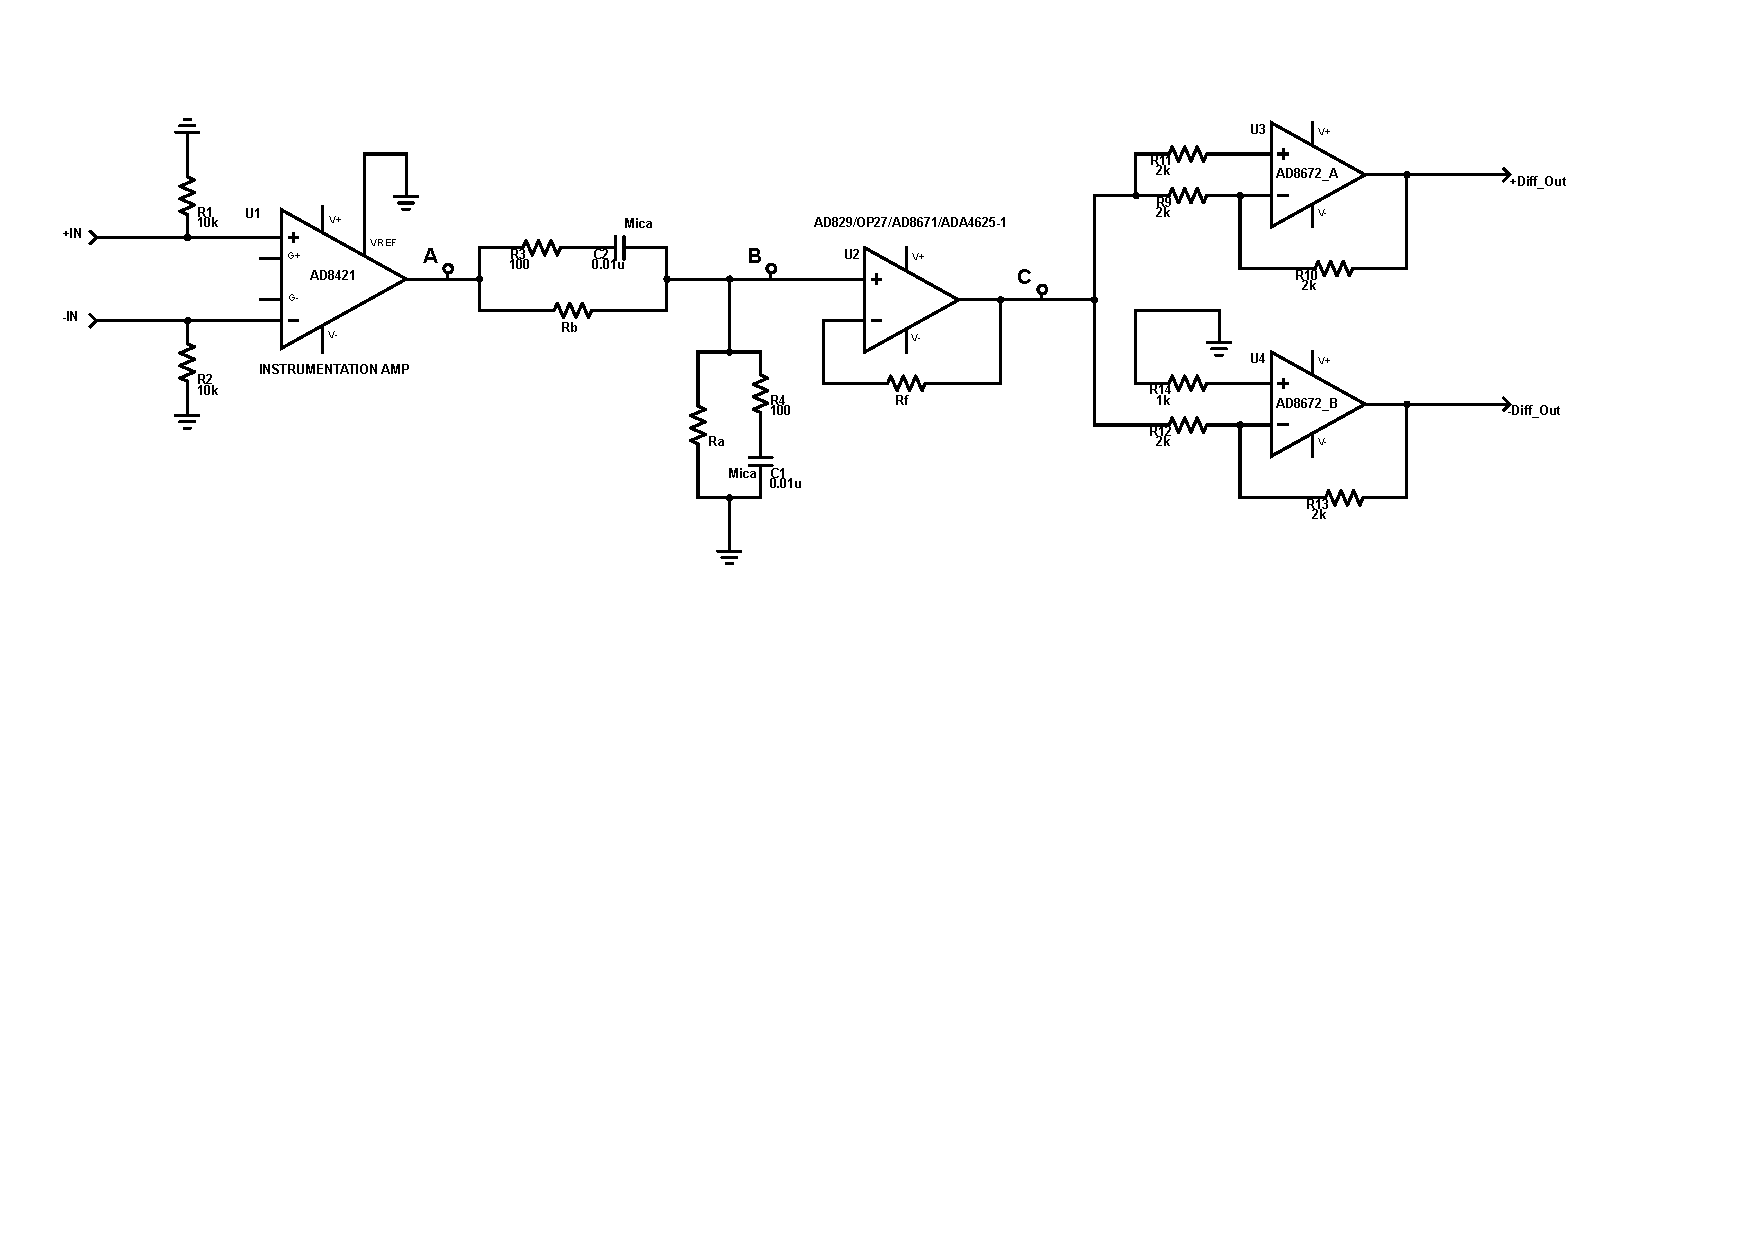
\includegraphics[angle=90, width=0.48\textwidth]{figure/DEWcircuit.pdf}
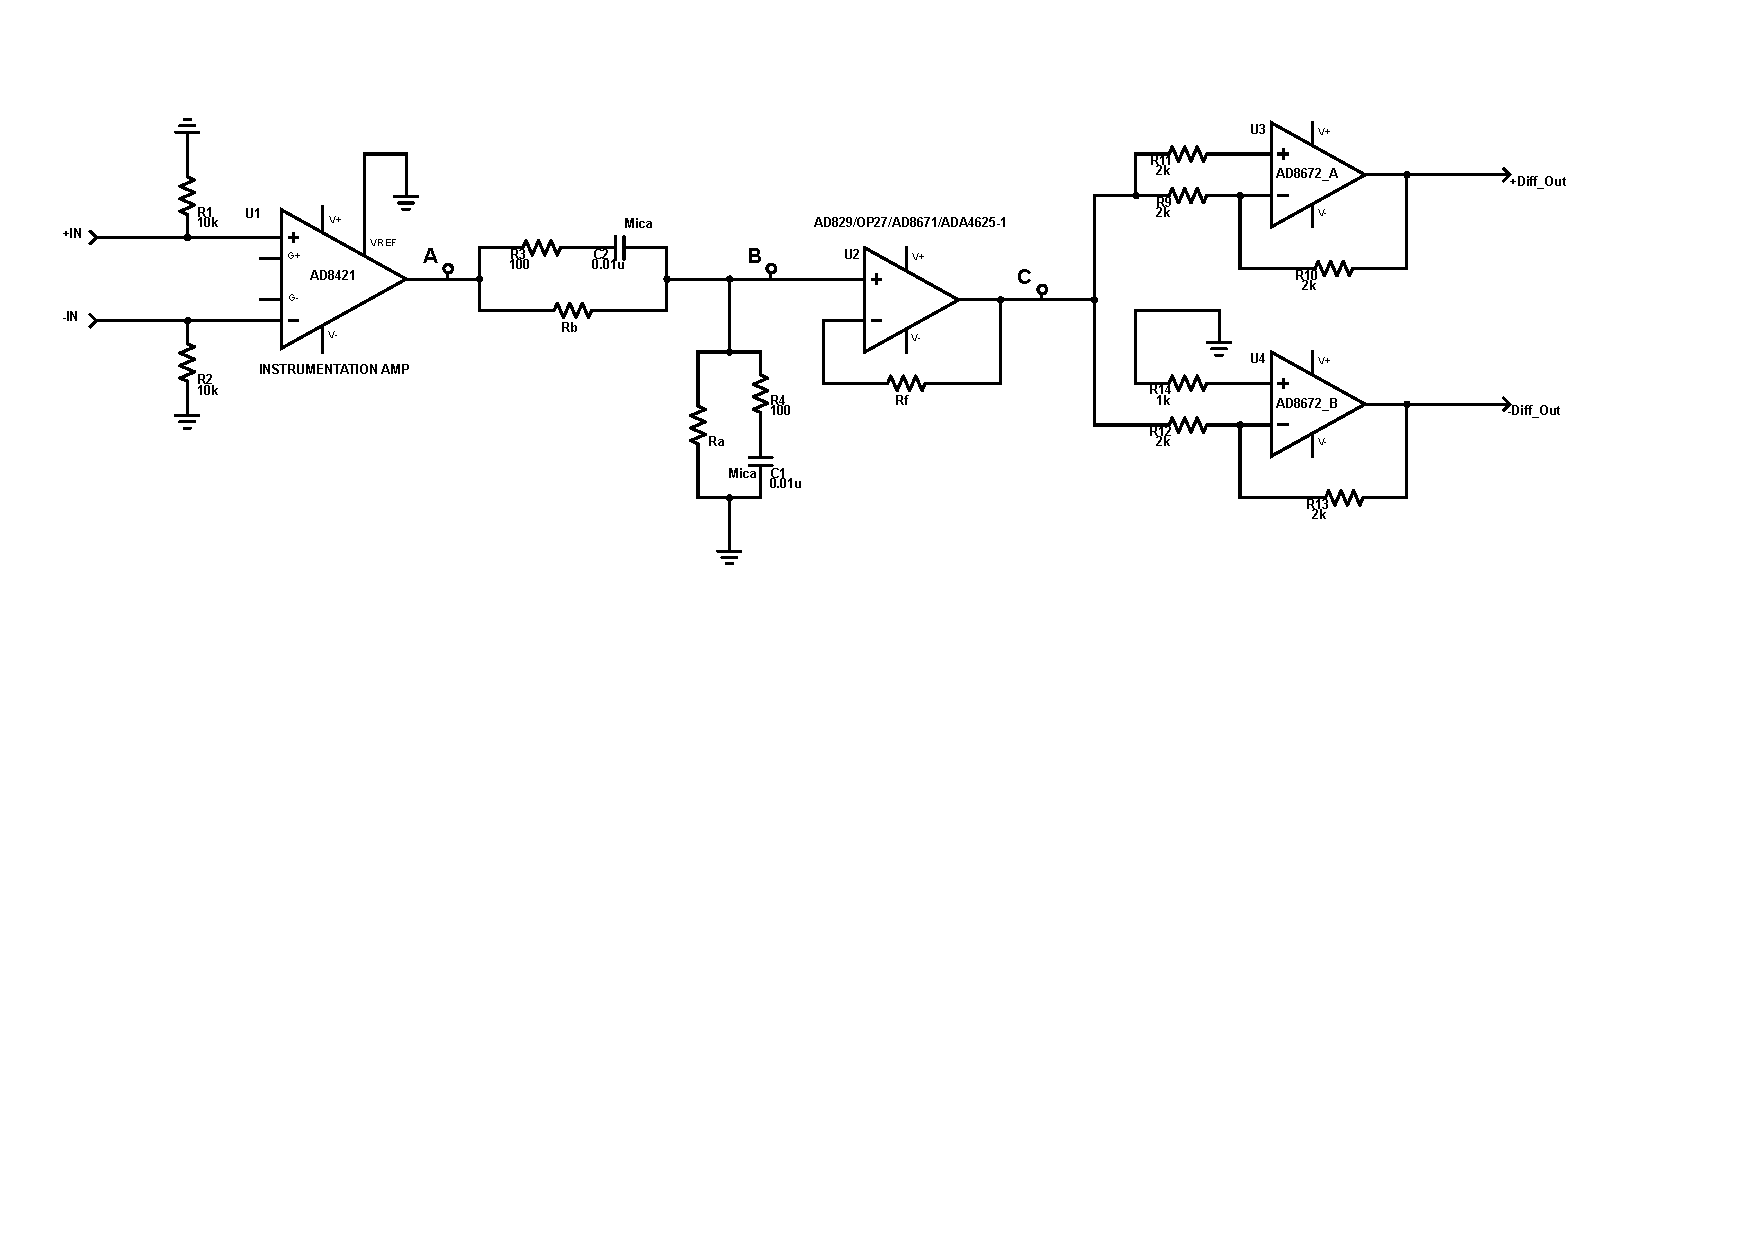
\includegraphics[width=1\textwidth]{figure/DEWcircuit.pdf}
\caption{De-Whitening filter circuit. }\label{fig:dewcircuit}
\index{figures}
\end{sidewaysfigure}
%\end{figure}


Problem of 16kHz excitation channel 
Implementation of 64kHz Excitation channel in KAGRA digital system

Principle of Analog filter
Design of De-Whitening filter
Performance test
Transfer function measurement 
Noise requirement
Create Inverse De-Whitening filter




